\chapter{Hardware of the Vision Correction Display}

We explore two hardware devices used for the vision-correction display: the pinhole mask and the lenslet array. Both devices are examples of light field displays.

\section{Light Field Display}
A light field is a vector function that describes the amount of light flowing in every direction through every point in space. The direction of each ray is given by the 5D plenoptic function $$L(x, y, z, \theta, \phi)$$, where (x, y, z) represents the position of the ray and $(\theta, \phi)$ represents the direction. The magnitude of the light ray is equivalent to its radiance, denoted by $L$ and measured in watts ($W$) per steradian ($sr$) per meter squared ($m^2$). The steradian is a measure of solid angle, or the subtended surface area on the unit sphere, and meters squared are used here to measure cross-sectional area.

\begin{figure}[ht]
  \centering
  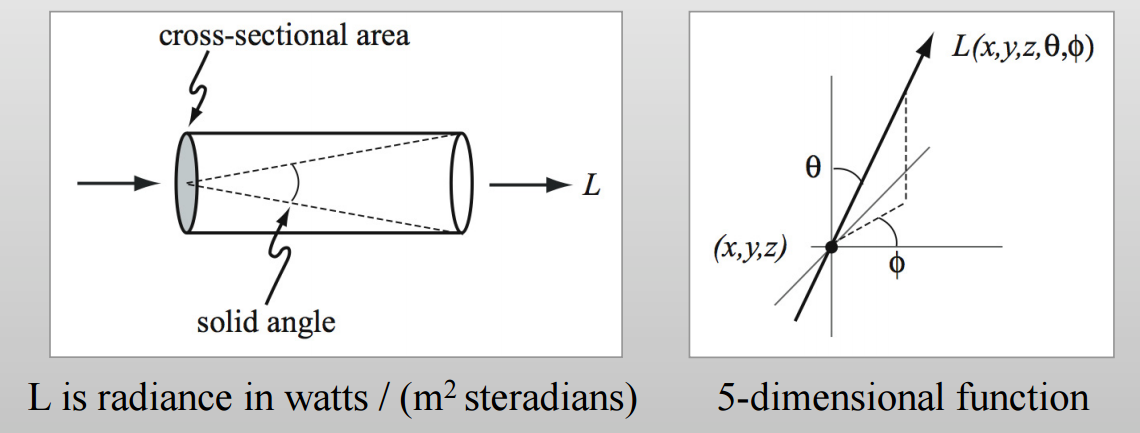
\includegraphics[width=5in]{chapters/chapter3/images/light_field.png}
  \caption{Radiance (left) and 5D plenoptic function (right) \cite{Stanford}}
  \label{fig:plenoptic}
\end{figure}

In the case of the vision correcting display, a 4D light field is considered. A 4D light field has constant radiance along the ray, and one dimension is ignored ($z$). Each light ray starts at a ($x, y$) coordinate on the screen and in the direction ($\theta, \phi$). The light field display is placed on top of the device and used to capture and/or manipulate the light fields from the surface.

% Maybe include a diagram here

\section{Pinhole Mask Display}

The pinhole mask display is a light field display that is composed of a sheet of black film taped to a layer of acrylic 6 millimeters thick. The black film is composed of a 2D array of pinholes in the shape shown in the figure below.

\begin{figure}[ht]
  \centering
  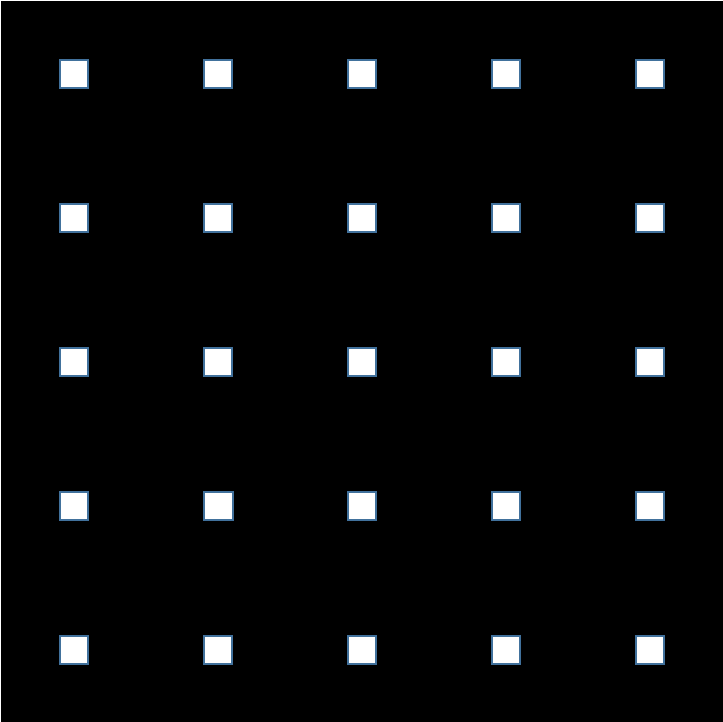
\includegraphics[width=3.5in]{chapters/chapter3/images/pmask.png}
  \caption{Area blocked and covered by pinhole.}
  \label{fig:pinhole}
\end{figure}

The pinhole mask is an example of a parallax barrier. The parallax barrier attenuates most of the light rays in the area covered by the pinhole. Therefore, less light rays will interfere, and light from each pixel will land on a smaller area on the retina. The blur as a result of defocus is reduced and contrast is improved. 

\begin{figure}[ht]
  \centering
  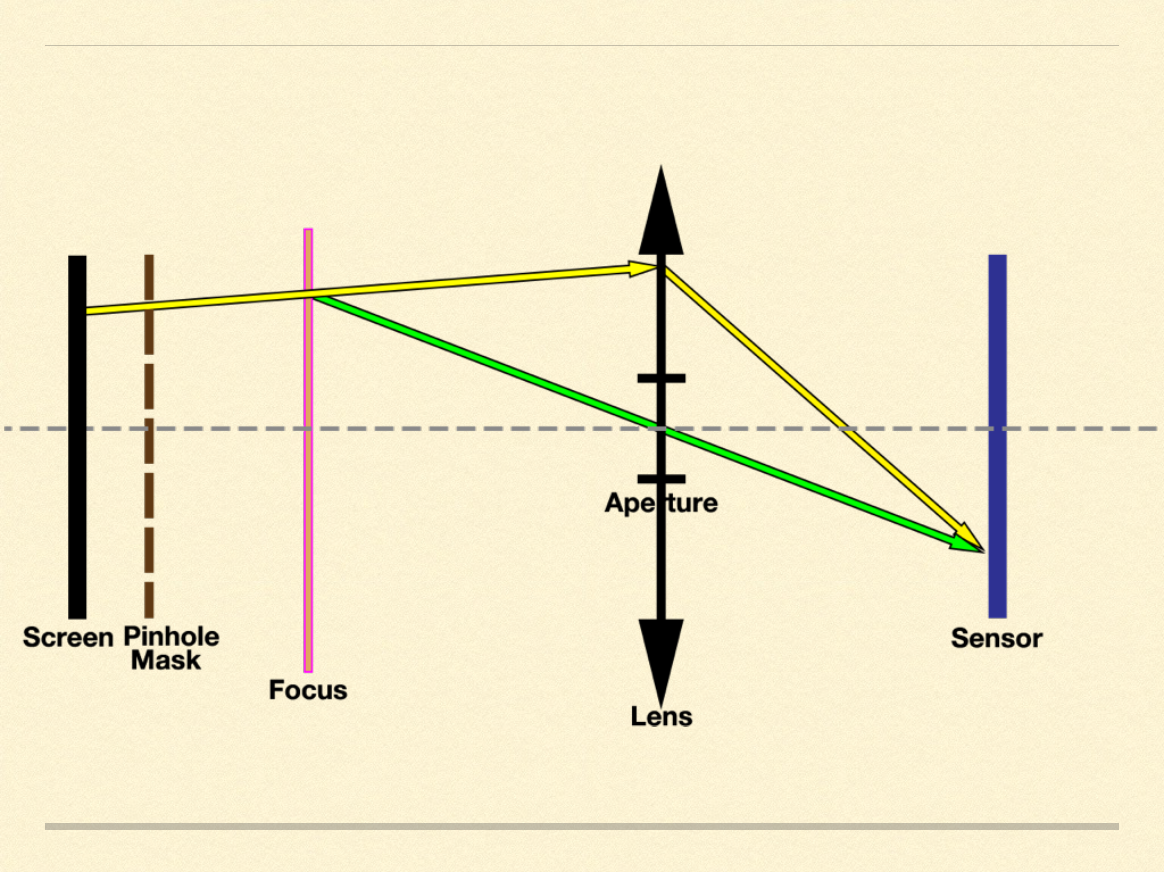
\includegraphics[width=5.0in]{chapters/chapter3/images/pinhole_rays.png}
  \caption{Light rays traveling through a pinhole \cite{Wu:EECS-2016-67}}
  \label{fig:pinhole_light}
\end{figure}

Previously, Huang et al. 2014 \cite{Huang:2014:VisionCorrectingDisplay} developed a similar pinhole mask display. Both Huang's display and our display had pinholes of size 75 micrometers that are 390 micrometers apart. Huang's display is used for the Apple iPod touch 4th generation display, which has a pixel pitch of 78 micrometers and resolution of $960 \times 640$ pixels, while our display is used for the iPhone 6, which has a resolution of $1334 \times 750$ pixels. Our pinhole mask has a greater depth (6 mm instead of 4 mm), and this increased depth allowed the outer pixels in the $5x5$ superpixel covered by the pinhole to become more visible. The light rays from the outer pixels travel at an angle through the pinhole mask and will miss the pupil or aperture if the angle was too large.


\section{Lens Array Display}

The lens array display is a 2D array of microlenses etched on a layer semiconductor material. A microlens is a small lens, generally with a diameter less than a millimeter ($mm$) and often as small as 10 micrometers ($\mu m$). The depth of the microlens is equal to the its focal length so that all of the light rays emanating from a screen pixel travel outwards in parallel. The size of the microlens is equal the length of its covered superpixel. For example, in a 5x5 superpixel on the iPhone6 (pixel size $0.078 mm$), the diameter of the microlens would be $5 \times 0.078mm = 0.3895mm$.  

\begin{figure}[ht!]
  \centering
  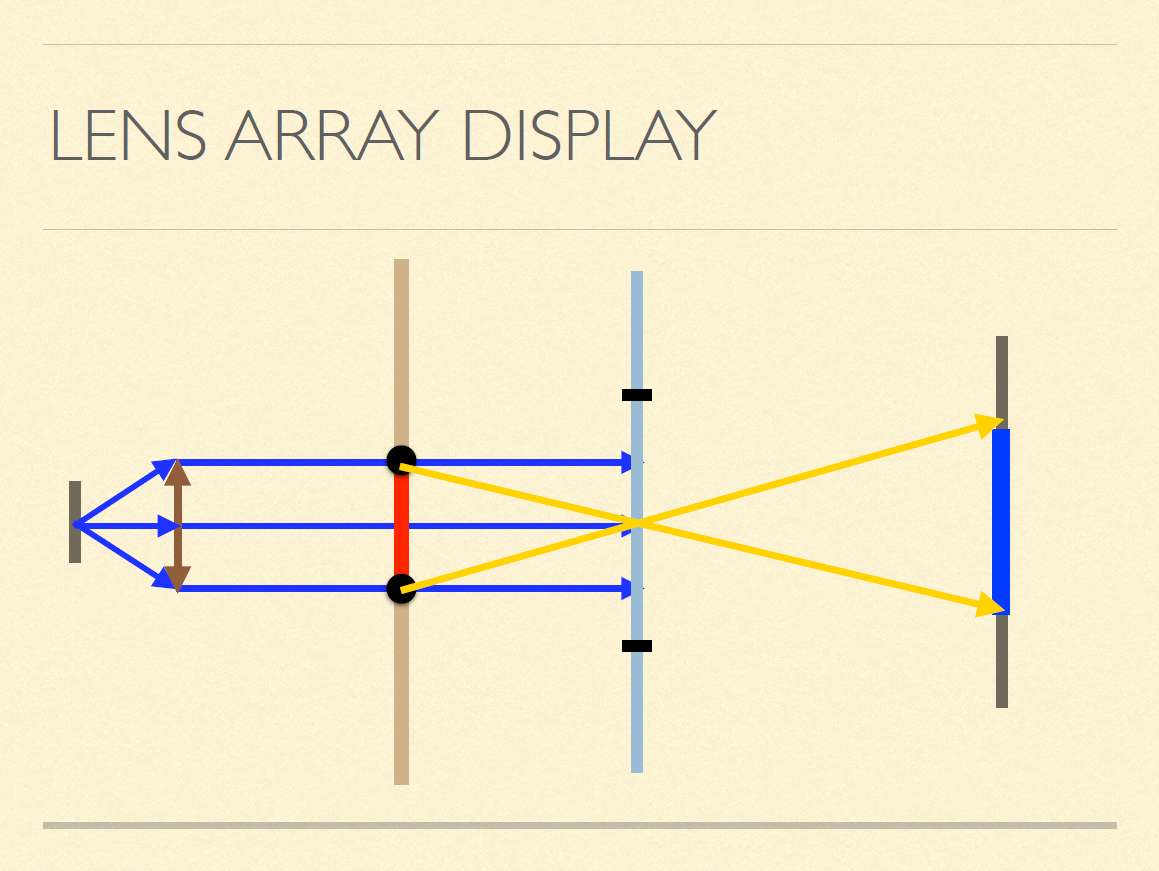
\includegraphics[width=5.0in]{chapters/chapter3/images/lens_rays.png}
  \caption{Light rays traveling through a microlens \cite{Wu:EECS-2016-67}}
  \label{fig:lens}
\end{figure}


One advantage of the lens array is that no light is lost and no information is lost. In the pinhole mask, light from many screen pixels are blocked, and only about 4 percent of all light under a 5x5 superpixel pass through the pinhole. However, in a microlens array, light from every screen pixel is allowed to pass through. One disadvantage of the microlens array is that it costs significantly more to manufacture than the pinhole mask display.

